% Metódy inžinierskej práce

\documentclass[10pt,twoside,slovak,a4paper]{article}

\usepackage[slovak]{babel}
\usepackage[IL2]{fontenc} % lepšia sadzba písmena Ľ než v T1
\usepackage[utf8]{inputenc}
\usepackage{graphicx}
\usepackage{url} % príkaz \url na formátovanie URL
\usepackage{hyperref} % odkazy v texte budú aktívne (pri niektorých triedach dokumentov spôsobuje posun textu)

\usepackage{cite}
%\usepackage{times}

\pagestyle{headings}

\title{Extrakcia informácii z webu pre analýzu dát pomocou Python\thanks{Semestrálny projekt v predmete Metódy inžinierskej práce, ak. rok 2023/24, vedenie: Ing. Mohammad Yusuf Momand, MSc.}} % meno a priezvisko vyučujúceho na cvičeniach

\author{Štefan Kučerák\\[2pt]
	{\small Slovenská technická univerzita v Bratislave}\\
	{\small Fakulta informatiky a informačných technológií}\\
	{\small \texttt{xkucerak@stuba.sk}}
	}

\date{\small 5. október 2023} % upravte



\begin{document}

\maketitle
%Čím sa zaoberáte a prečo (ako to definujú iní a ako by ste to definovali vy)?
%Aký je stav v oblasti (s odkazmi na zdroje)?
%Čo pokladáte za významný problém v tejto oblasti a prečo (opora v literatúre)?
%Je nejaké riešenie a aké?
%Je vaše riešenie podobné iným (hoci aj z inej oblasti a len v z určitého hľadiska)?
%O čom je článok, k čomu ste ním prispeli a čo zostáva otvorené?


\begin{abstract}
Extrakcia informácii z webu v angličtine označovaná ako "Web scraping" je automatický spôsob získavania údajov zo stránky. Umožňuje získať presné informácie v krátkom čase. Získané dáta sú pripravené na ďalšie spracovane.

%Stranky urcene len pre ludi ... dostat data ... na spracovanie ... stroj nezaujima vizual stranka ... 
\end{abstract}



\section{Úvod}

Webstránky sú prevažne určené pre ľudí a tomu zodpovedá aj ich grafický dizajn. Ak chceme použiť hodnotné informácie z webstránky pre našu aplikáciu nastáva problém z ich extrakciou. Manuálna extrakciou týchto informácii by bola časovo náročná a s veľkou pravdepodobnosťou by nastala chyba pri kopírovaní. Riešením tohoto problému je automatizovaný zber informácii, ktorý priblížim v nasledujúcom článku. Celý proces extrakcie dát sa dá vyhotoviť pomocou rôznych programovacích jazykov. Pre tento článok som vybral programovacom jazyku Python, pretože je v dnešnej dobe dosť populárny a využíva sa v oblasti analýzy dát.


Vysvetlenie princípu extrakcie dát z webu je v časti~\ref{webscraping}. V časti~\ref{usecase} sú príklady využitia tejto metódy v reálnom svete. Knižnice pre extrakciu dát sú v časti~\ref{kniznice} a príklad implementácie pomocou jednej z knižníc je v časti~\ref{imp}.

(poznámka: Článok je stále v príbehu písania, zatiaľ sú skôr zachytené myšlienky, ktoré by som chcel použiť. Vety ešte nie sú úplne správne sformulované. Môj východzí článok je: \cite{10145369})

\section{Web Scraping}\label{webscraping}

Cieľom je získať dáta a následne ich analyzovať, napríklad pre výhodu na trhu. Získavanie dát je zložitý proces obsahujúci viacej krokov začínajúc výberom aké dáta vlastne chceme zbierať, ich usporiadaním, odstraňovaním nesprávnych dát, opätovnou analýzou použitím algoritmov\cite{8822022}.
Získavanie veľkého množstva dát pomocou ľudskej sily by bolo veľmi obtiahne a vzniká priestor na chybu\cite{10145369}. Tento problém rieši Web Scraping a to tak že pomocou automatizácie je možne získavať tieto dáta rýchlejšie a univerzálnejšie. Web scraping je používaný spoločnosťami ale aj jednotlivcami, ktorý chcú využiť voľne dostupné informácie\cite{10145369}. Príklady jeho využitia sú napríklad: sledovanie ceny výrobku, návštevnosti stránky,  čítanie komentárov na stránke, zistenie hypertextových odkazov na danej stránke a mnoho ďalších\cite{10250745}.

\begin{figure*}[tbh]
    \centering
    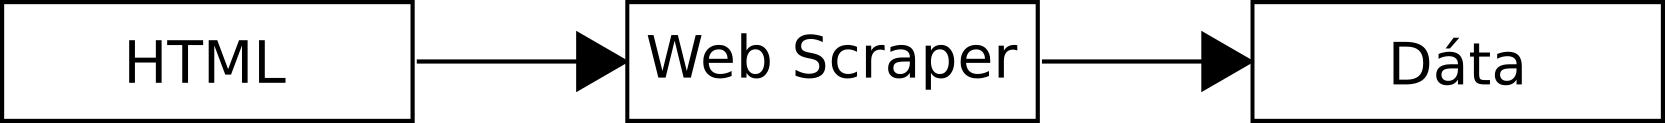
\includegraphics[width= 0.9\textwidth]{diag.png}
    \caption{Princíp extrakcie}
    \label{f:diagram}
\end{figure*}

Web scraper v tomto prípade knižnica pre Python stojí medzi html stránkou a dátami o ktoré máme záujem (Obr.~\ref{f:diagram}). Na začiatku musíme mať nejakú cieľovú stránku z ktorej chceme dáta získať. Scrapery vyhľadávajú v html podla html tagov ako napríklad: h1, div, span\cite{9215357}.

%\cite{10145369} Web Scraping for Data Analytics: A BeautifulSoup Implementation
%\cite{10250745} An Extensive Review on Web Scraping Technique using Python
%\cite{8822022} Data Analysis by Web Scraping using Python
%\cite{9215357} A Survey on Python Libraries Used for Social Media Content Scraping

\section{Príklady reálneho využitia tejto metódy}\label{usecase}
Jedným z príkladov je článok "Phishing Web Page Detection using web Scraping“ \cite{10115148}, v ktorom sa zaoberajú automatizovaným odhaľovaním phishing stránok. Ich riešenie na odhaľovanie takýchto stánok má presnosť detekcie viac ako 98\%. Pri tomto projekte bol požitý Python a knižnica Beautiful Soup(časť~\ref{kniznice}).

Ďalším z pŕikladov je článok "Food Genie, Recipe Search Algorithm using Web Scraping"\cite{10270597}, ktorý využiva web scraping na porovnanie indegriencíi, ktoré majú ísť do rovnakého receptu. Rieši problém toho že naprieč rôznymi stránkami má recept iný postup alebo sú použité iné suroviny. Napríklad pri tomto projekte bol využitý Python a knižnica scrapy(časť~\ref{kniznice}).

Ako posledný príklad by som uviedol článok "NEWSONE- AN AGGREGATION SYSTEM FOR NEWS USING WEB SCRAPING METHOD"\cite{8067594}, ktorý požíva web scraping na extrakciu správ z rôznych web stránok v rôznych jazykoch a sústreďuje ich na platformu "NewsOne". Pri tomto projekte sa taktiež využíva Python a knižnica Beautiful Soup(časť~\ref{kniznice}).

\section{Knižnice pre získavanie dát} \label{kniznice}
Zoznam knižníc, ktoré môžu byť použité na extrakciu dát z webu pre programovací jazyk Python:
\begin{itemize}
\item Requests\footnote{\url{https://pypi.org/project/requests/}} je jednoduchá knižnica ktorá umožňuje vytvoriť http požiadavky a to post aj get. Táto knižnica je najčastejšie používaná na získanie html zo stánky. Ak by sme chceli použiť len samotnú knižnicu museli by sme si na vyhľadávanie napísať vlastný algoritmus.
\item Beautiful Soup\footnote{\url{https://pypi.org/project/beautifulsoup4/}} táto knižnica obsahuje nástroje na vyhľadávanie, upravovanie a iteráciu v html alebo xml. Podmienkou pre fungovanie je vstup vo formáte html alebo xml a pre ten sa najčastejšie využíva knižnica Requests.
\item Scrapy\footnote{\url{https://pypi.org/project/Scrapy/}} je rýchly framework pre prehľadávanie webu na vysokej úrovni, ktorý sa používa na prehľadávanie webových stránok a extrahovanie štruktúrovaných údajov. Dá sa použiť na širokú škálu účelov, od získavania dát až po monitorovanie a automatizované testovanie. Výhodou oproti Beautiful Soup je že knižnica obsahuje nástroj na extrakciou html zo stránky.
\item Selenium\footnote{\url{https://pypi.org/project/selenium/}} je knižnica, ktorá umožňuje priamo pomocou prehliadača interagovať so stránkami. Podporované prehliadače Firefox, Chrome, Internet Explorer. %pomocou scrit
%\item Lxml\footnote{\url{https://pypi.org/project/lxml/}}
%\item Urllib3\footnote{\url{https://pypi.org/project/urllib3/}}
\item MechanicalSoup\footnote{\url{https://pypi.org/project/MechanicalSoup/}} Knižnica na automatizáciu interakcie s webovými stránkami. MechanicalSoup automaticky ukladá a odosiela súbory cookie, sleduje presmerovania a môže sledovať odkazy a odosielať formuláre. Avšak nepodporuje JavaScript.
\end{itemize}
%Všetky uvedené knižnice sú oppensource a free.

\section{Jednoduchý príklad požitím knižnice Beautiful Soup} \label{imp}

\begin{figure*}[tbh]
    \centering
    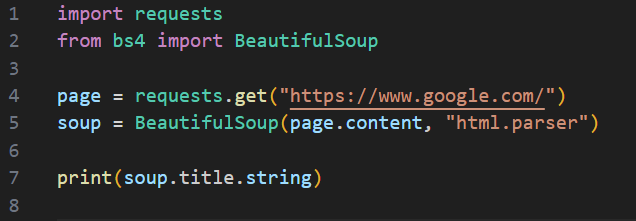
\includegraphics[width= 0.9\textwidth]{code.png}
    \caption{Program}
    \label{f:code}
\end{figure*}

Na Obr.~\ref{f:code} je príklad kódu, ktorý zo stránky \url{https://www.google.com/} extrahuje názov stánky a teda tag title. Ako prvé sa spraví požiadavka pomocou knižnice Requests, ktorá vráti web stránku vo formáte html. Na html sa použije knižnica Beautiful Soup, ktorá vie pracovať s jednotlivými tagmi v html súbore. Knižnici dáme požiadavkou na vypísanie názvu stránky v reťazci. Následne dostaneme výstup "Google". Tento princíp je uvedený v Obr.~\ref{f:diagram}. Podobný postup sa dá využiť aj napríklad na sledovanie ceny produktu a to tak že nájdeme html tag, ktorý obsahuje symbol meny a teda aj číselnú hodnotu.

%priklad bude na extrakciu ceny z nejakeho znameho eshpu


\section{Záver} \label{zaver} % prípadne iný variant názvu
Výsledkom mojej práce je článok ktorý približuje tému extrakcie informácii z webu pomocou programovacieho jazyka Python. A taktiež projekt na predmet Metódy inžinierskej prace.


\paragraph{Spoločenské súvislosti.}

\paragraph{Historické súvislosti.}

\paragraph{Technológia a ľudia.}

\paragraph{Udržateľnosť a etika.}
Tento spôsob získavania informácii môže byt neetický, pretože stránka môže predávať svoje dáta za peniaze a tak obchádzame tuto peňažnú bariéru. Týmto problémom sa zaoberajú mnohý ľudia a jedným z príkladov je článok\cite{10092327}., ktorý navrhuje rôzne spôsoby ako zabrániť extrakcii dát.

%\cite{10092327} Solution to Web Scraping


% týmto sa generuje zoznam literatúry z obsahu súboru literatura.bib podľa toho, na čo sa v článku odkazujete
\bibliography{literatura}
\bibliographystyle{plain} % prípadne alpha, abbrv alebo hociktorý iný
\end{document}
